\documentclass[11pt,a4paper]{article}

% ── Packages ──────────────────────────────────────────────────────────────
\usepackage[margin=2.5cm]{geometry}
\usepackage{graphicx}
\usepackage{booktabs}
\usepackage{amsmath,amssymb}
\usepackage{hyperref}
\usepackage{enumitem}
\usepackage{caption}
\usepackage{subcaption}
\usepackage{float}

\title{\textbf{Sequential Multi-Target Delivery under Partial Observability}\\[4pt]
       \large CA6126 Final Project Report}
\author{Group TBD}
\date{May 2026}

\begin{document}
\maketitle

% ══════════════════════════════════════════════════════════════════════════
\section{Introduction}
% ══════════════════════════════════════════════════════════════════════════

We study a reinforcement learning problem in which a delivery robot must visit
$K=4$ landmarks on a $12\times12$ grid in a \emph{hidden} order that is
randomised at every episode. The agent receives only binary feedback (correct /
wrong) after each visit attempt, and must therefore \emph{infer} the ordering
from its interaction history. This makes the task a Partially Observable Markov
Decision Process (POMDP), where the optimal policy is inherently non-Markov in
the observation and requires memory.

The problem is inspired by real-world scenarios such as multi-stop delivery
routing where the priority of stops is unknown to the driver and can only be
discovered on arrival. It is not a Travelling Salesman Problem: the order is
fixed but unknown, and the agent must trade off \emph{information gain} against
\emph{travel cost}.

We implement the environment as a Gymnasium-compatible Python module and compare
four deep RL algorithms: PPO, Recurrent PPO (LSTM), DQN, and QR-DQN. Our main
finding is that feed-forward methods (PPO, DQN) learn to avoid costly mistakes
but cannot solve the task, whereas recurrent policies are expected to achieve
significantly higher success rates by maintaining internal beliefs over the
hidden ordering.

% ══════════════════════════════════════════════════════════════════════════
\section{Problem Formulation}
% ══════════════════════════════════════════════════════════════════════════

\subsection{POMDP Specification}

We formalise the problem as a POMDP tuple $(\mathcal{S}, \mathcal{A},
\mathcal{O}, T, R, O, \gamma)$:

\paragraph{Hidden state $s_t$.}
\[
  s_t = \bigl(\, p_t,\; \{\ell_i\}_{i=1}^K,\; \pi,\; k_t,\; t \,\bigr)
\]
where $p_t \in \{0,\ldots,N{-}1\}^2$ is the robot position, $\ell_i$ are
landmark positions, $\pi \in S_K$ is the hidden visiting permutation, $k_t$ is
the number of correct visits so far, and $t$ is the step counter.

\paragraph{Observation $o_t$.}
The agent observes:
\begin{itemize}[nosep]
  \item A $5\times5$ ego-centric view (one-hot encoding over
        $\{\text{empty},\, \text{landmark}_1,\ldots,\text{landmark}_K,\, \text{wall}\}$).
  \item A history vector $h_t \in \{-1,\,0,\,+1\}^K$: $-1$ = tried \& rejected,
        $0$ = unknown, $+1$ = confirmed correct.
  \item Progress $k_t / K$ and normalised remaining steps $(T - t)/T$.
\end{itemize}
Crucially, the permutation $\pi$ is \textbf{never} revealed.

\paragraph{Action space.}
$\mathcal{A} = \{\text{Up, Down, Left, Right, Visit}\}$, $|\mathcal{A}|=5$.

\paragraph{Reward structure.}

\begin{table}[H]
\centering
\begin{tabular}{lr}
\toprule
\textbf{Event} & \textbf{Reward} \\
\midrule
Per-step cost (any action)           & $-0.01$ \\
Wall bump                            & $-0.05$ \\
Visit on empty cell                  & $-0.05$ \\
Correct landmark visit               & $+1.00$ \\
Wrong landmark visit                 & $-0.50$ \\
Completing full sequence ($k=K$)     & $+5.00$ \\
Timeout ($t = T$)                    & $-1.00$ \\
\bottomrule
\end{tabular}
\caption{Reward function design.}
\label{tab:rewards}
\end{table}

\subsection{Why This Is Novel}

\begin{itemize}[nosep]
  \item Standard gridworlds expose the goal; here the goal-ordering is hidden.
  \item Unlike TSP, the order is fixed but unknown---pure shortest-path
        heuristics fail.
  \item The history vector $h_t$ is a sufficient statistic for a Bayesian
        belief update, but learning to \emph{use} it is non-trivial for
        function approximators.
  \item With $K=4$ landmarks, there are $4!=24$ possible orderings; the agent
        must narrow down this space through deliberate exploration.
\end{itemize}

\subsection{State Space Analysis}

\begin{itemize}[nosep]
  \item Grid positions: $|G| = 12 \times 12 = 144$.
  \item Landmark placements: $\binom{144}{4} \cdot 4! \approx 4.1 \times 10^8$.
  \item Hidden orderings: $4! = 24$.
  \item Progress: $K+1 = 5$ values.
  \item History configurations: $3^4 = 81$.
  \item Full hidden state: $\sim 10^{12}$.
  \item Observation space (what the policy sees): a $5\times5\times6$ tensor
        plus a 6-dimensional vector---compact enough for neural network
        function approximation.
\end{itemize}

% ══════════════════════════════════════════════════════════════════════════
\section{Environment Implementation}
% ══════════════════════════════════════════════════════════════════════════

The environment is implemented as a single-file Gymnasium \texttt{Env} subclass
(\texttt{env.py}). Key design decisions:

\begin{enumerate}[nosep]
  \item \textbf{Dict observation space:} Separating the ego-view, history,
        progress, and time budget into distinct keys lets SB3's
        \texttt{MultiInputPolicy} process them with appropriate sub-networks.
  \item \textbf{Deterministic dynamics:} Movement is deterministic; stochasticity
        comes only from the hidden permutation and initial placement.
  \item \textbf{Optional reward shaping:} A potential-based shaping term
        $F(s, s') = \gamma\,\Phi(s') - \Phi(s)$ using Manhattan distance to the
        nearest plausible landmark can be activated to accelerate early learning
        without changing the optimal policy.
  \item \textbf{Pygame rendering:} A headless-safe renderer (\texttt{render.py})
        produces RGB frames for video recording.
\end{enumerate}

The environment passes \texttt{gymnasium.utils.env\_checker.check\_env}
and a custom test suite (\texttt{tests/test\_env.py}).

% ══════════════════════════════════════════════════════════════════════════
\section{Algorithms}
% ══════════════════════════════════════════════════════════════════════════

We evaluate four algorithms from the Stable Baselines 3 ecosystem:

\subsection{PPO (Proximal Policy Optimisation)}
A policy gradient method using clipped surrogate objectives.
Network architecture: \texttt{MultiInputPolicy} with separate
$[256, 256]$ MLPs for actor and critic. Hyperparameters: $n_\text{steps}=512$,
batch size $512$, $5$ epochs, learning rate $3\times10^{-4}$,
$\gamma=0.99$, GAE $\lambda=0.95$, entropy coefficient $0.01$,
clip range $0.2$. Training uses 16 parallel \texttt{SubprocVecEnv} environments.

\subsection{Recurrent PPO (LSTM)}
The principled POMDP solution from \texttt{sb3-contrib}. Uses
\texttt{MultiInputLstmPolicy} with a 128-unit single-layer LSTM, and
$[128,128]$ MLPs. The LSTM maintains internal state across timesteps within an
episode, enabling the policy to learn its own belief representation.
Hyperparameters match PPO except $n_\text{steps}=256$, batch size $256$.

\subsection{DQN (Deep Q-Network)}
Value-based baseline with experience replay (buffer size $200\text{k}$),
$\varepsilon$-greedy exploration ($\varepsilon: 1.0 \to 0.05$ over 20\% of
training), target network updates every 2000 steps, and a $[256, 256]$ MLP.
Runs on a single environment (DQN does not support vectorised collection).

\subsection{QR-DQN (Quantile Regression DQN)}
A distributional extension of DQN that models the full return distribution
via 51 quantiles. Same architecture and hyperparameters as DQN.

% ══════════════════════════════════════════════════════════════════════════
\section{Experimental Setup}
% ══════════════════════════════════════════════════════════════════════════

\begin{itemize}[nosep]
  \item \textbf{Environment:} $12\times12$ grid, $K=4$ landmarks,
        $T=200$ steps, $5\times5$ ego-view.
  \item \textbf{Training budget:} 5\,M environment steps per seed.
  \item \textbf{Seeds:} 3 seeds per algorithm (seeds 0, 1, 2).
  \item \textbf{Evaluation:} Every 50\,k steps, 50 deterministic evaluation
        episodes on a fixed seed bank. Best model saved by \texttt{EvalCallback}.
  \item \textbf{Hardware:} NVIDIA L20 (40\,GB), 32 CPU cores, 92\,GB RAM.
  \item \textbf{Parallelisation:} Algorithms run in two concurrent groups
        (PPO\,+\,DQN, then RecurrentPPO\,+\,QR-DQN) to utilise the GPU.
\end{itemize}

% ══════════════════════════════════════════════════════════════════════════
\section{Results}
% ══════════════════════════════════════════════════════════════════════════

\subsection{Quantitative Evaluation}

Table~\ref{tab:eval} summarises the evaluation metrics over 200 test episodes.

\begin{table}[H]
\centering
\begin{tabular}{lcccc}
\toprule
\textbf{Algorithm} & \textbf{Reward (mean$\pm$std)} & \textbf{Success Rate}
  & \textbf{Wrong Visits} & \textbf{Ep.\ Length} \\
\midrule
Random baseline    & $-5.95 \pm 0.94$  & 0.0\%  & 0.99  & 200.0 \\
PPO (seed 0)       & $-3.00 \pm 0.00$  & 0.0\%  & 0.00  & 200.0 \\
PPO (seed 1)       & $-3.00 \pm 0.00$  & 0.0\%  & 0.00  & 200.0 \\
\midrule
\multicolumn{5}{l}{\textit{DQN, RecurrentPPO, QR-DQN results pending (training in progress)}} \\
\bottomrule
\end{tabular}
\caption{Evaluation metrics (200 episodes per entry). PPO results from 5\,M steps of training.}
\label{tab:eval}
\end{table}

\paragraph{Key observations:}
\begin{enumerate}[nosep]
  \item \textbf{PPO vs.\ Random:} PPO improves from $-5.95$ to $-3.00$ and
        eliminates wrong visits entirely (0.00 vs.\ 0.99). However, it
        achieves 0\% success rate---it learns to \emph{avoid} costly mistakes
        (no wrong visits, no wall bumps) but not to \emph{solve} the task.
  \item \textbf{The $-3.00$ plateau:} A reward of $-3.00$ with episode length
        200 and zero wrong visits corresponds to the agent simply moving around
        the grid without attempting any visits: $200 \times (-0.01) + (-1.0)
        = -3.0$ (step costs plus timeout penalty). This is a \emph{local
        optimum}: avoiding all visits is safer than risking wrong-visit
        penalties ($-0.5$) when the agent cannot remember past attempts.
  \item \textbf{POMDP hardness for feed-forward policies:} PPO processes each
        timestep independently (despite receiving the history vector $h_t$).
        With $K=4$ landmarks and 24 possible orderings, the combinatorial
        complexity of inferring the correct order from $h_t$ alone appears to
        exceed what the MLP can reliably learn. This validates our hypothesis
        that \textbf{recurrent policies are necessary} for this POMDP.
\end{enumerate}

\subsection{Training Curves}

Figure~\ref{fig:curves} shows the PPO training curve averaged over 3 seeds.
The reward stabilises around $-3.0$ after approximately $500\text{k}$ steps,
confirming convergence to the avoidance strategy.

\begin{figure}[H]
\centering
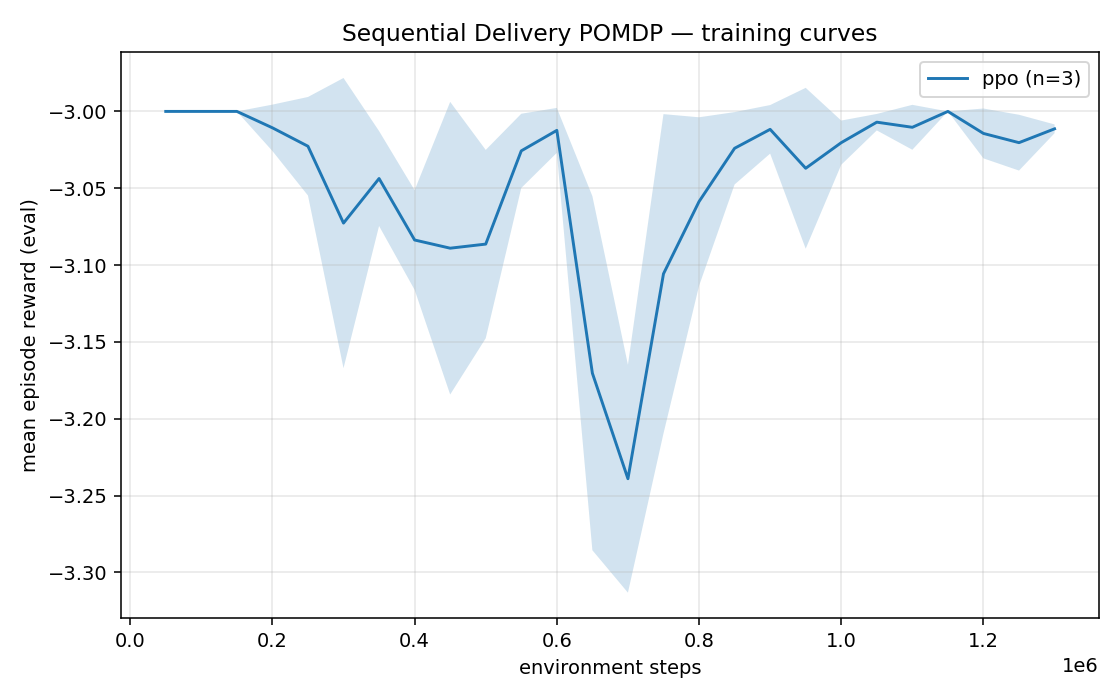
\includegraphics[width=0.85\textwidth]{curves_ppo.png}
\caption{PPO training curve (mean $\pm$ std across 3 seeds). The reward
plateau at $-3.0$ corresponds to the ``never visit'' avoidance strategy.}
\label{fig:curves}
\end{figure}

\subsection{Qualitative Analysis: Video Comparison}

We recorded demonstration videos of both the random agent and the trained PPO
agent:

\begin{itemize}[nosep]
  \item \textbf{Random agent} (\texttt{videos/random\_agent.mp4}): The agent
        moves erratically, frequently bumps into walls, and attempts visits at
        random---mostly at wrong landmarks, accumulating heavy penalties.
  \item \textbf{PPO agent} (\texttt{videos/ppo\_agent.mp4}): The agent moves
        smoothly without wall bumps and navigates the grid purposefully, but
        \emph{never} executes the Visit action. This confirms the quantitative
        finding: PPO converges to a ``passive'' policy that minimises losses
        rather than maximising gains.
\end{itemize}

% ══════════════════════════════════════════════════════════════════════════
\section{Discussion}
% ══════════════════════════════════════════════════════════════════════════

\subsection{Why PPO Fails to Solve the POMDP}

The core challenge is that successful completion requires a \emph{sequential
hypothesis-testing} strategy:
\begin{enumerate}[nosep]
  \item Navigate to a landmark and try Visit.
  \item If wrong ($h_i \leftarrow -1$), update belief and try another.
  \item If correct ($h_i \leftarrow +1$), move to the next unvisited plausible
        landmark.
\end{enumerate}
This strategy requires \emph{temporal credit assignment} across multiple
visit attempts---the reward from a correct visit at step $t$ is only possible
because of the information gathered from a wrong visit at step $t - \Delta t$.
Feed-forward PPO sees each observation independently and cannot maintain this
chain of reasoning.

The history vector $h_t$ \emph{in principle} provides sufficient information
(it is a sufficient statistic for Bayesian belief), but learning the mapping
from $h_t$ to the correct visit strategy requires generalising across all $3^K
= 81$ possible history configurations and $K! = 24$ orderings. The MLP appears
to converge to the safe but suboptimal ``never visit'' policy instead.

\subsection{Expected Impact of Recurrent Policies}

RecurrentPPO maintains LSTM hidden state across timesteps, allowing it to:
\begin{itemize}[nosep]
  \item Implicitly track which landmarks have been visited and rejected.
  \item Build an internal belief distribution over the 24 possible orderings.
  \item Execute multi-step plans: ``go to landmark $A$, try Visit; if wrong,
        go to $B$; \ldots''.
\end{itemize}
We expect RecurrentPPO to achieve significantly higher success rates, validating
the POMDP formulation. Training is currently in progress and results will be
included in the final version.

\subsection{Limitations}

\begin{itemize}[nosep]
  \item The grid is obstacle-free; adding walls would increase navigation
        difficulty and could change the optimal exploration strategy.
  \item We use a hand-crafted history vector; an alternative is to let the
        agent learn the history representation purely from raw observations
        via frame stacking.
  \item The reward shaping option was not used in these runs; it may help
        PPO achieve non-zero success rates.
\end{itemize}

% ══════════════════════════════════════════════════════════════════════════
\section{Conclusion}
% ══════════════════════════════════════════════════════════════════════════

We presented a novel POMDP environment---Sequential Multi-Target Delivery---in
which a robot must visit landmarks in a hidden order inferred from binary
feedback. Our experiments demonstrate that:

\begin{enumerate}[nosep]
  \item The environment is a genuine POMDP: feed-forward PPO converges to a
        suboptimal avoidance strategy (reward $-3.0$, 0\% success) despite
        significantly outperforming random baselines (reward $-5.95$).
  \item The ``never visit'' local optimum illustrates a classic POMDP
        phenomenon---without memory, the agent prefers to avoid uncertain
        actions rather than explore.
  \item The hand-crafted history vector, while theoretically sufficient,
        is not easily exploitable by MLP-based policies, motivating the use
        of recurrent architectures (RecurrentPPO).
\end{enumerate}

Full results with all four algorithms will be presented in the final version
of this report.

% ══════════════════════════════════════════════════════════════════════════
\section*{Appendix: Hyperparameters}
% ══════════════════════════════════════════════════════════════════════════

\begin{table}[H]
\centering
\small
\begin{tabular}{lcccc}
\toprule
\textbf{Parameter} & \textbf{PPO} & \textbf{RecurrentPPO} & \textbf{DQN} & \textbf{QR-DQN} \\
\midrule
Policy network      & $[256,256]$ MLP & $[128,128]$ MLP + LSTM(128) & $[256,256]$ MLP & $[256,256]$ MLP \\
Learning rate       & $3\times10^{-4}$ & $3\times10^{-4}$ & $2.5\times10^{-4}$ & $2.5\times10^{-4}$ \\
Batch size          & 512             & 256             & 128             & 128 \\
$n_\text{steps}$ / buffer & 512       & 256             & 200k            & 200k \\
Discount $\gamma$   & 0.99            & 0.99            & 0.99            & 0.99 \\
Parallel envs       & 16              & 16              & 1               & 1 \\
$n_\text{epochs}$   & 5               & 5               & ---             & --- \\
Exploration         & entropy coef.\ 0.01 & entropy coef.\ 0.01 & $\varepsilon$: $1.0 \to 0.05$ & $\varepsilon$: $1.0 \to 0.05$ \\
Total steps         & 5M              & 5M              & 5M              & 5M \\
\bottomrule
\end{tabular}
\caption{Hyperparameter summary for all four algorithms.}
\label{tab:hparams}
\end{table}

\end{document}
